\documentclass [letterpaper,11pt,twoside]{article}
%\usepackage{pst-pdf,pst-text,pstricks-add}
\providecommand{\ifincludeall}{\iffalse}
\usepackage{fancyhdr}
\usepackage{lastpage}
\usepackage{enumerate}
\ifincludeall

  \usepackage{wrapfig}

%================================ Unicode ================================
  \usepackage[utf8]{inputenc}
  \DeclareUnicodeCharacter{916}{\ensuremath{\Delta}}
  \DeclareUnicodeCharacter{937}{\ensuremath{\Omega}}
  \DeclareUnicodeCharacter{949}{\ensuremath{\epsilon}}
  \DeclareUnicodeCharacter{956}{\ensuremath{\mu}}
  \DeclareUnicodeCharacter{963}{\ensuremath{\sigma}}
  \DeclareUnicodeCharacter{977}{\ensuremath{\theta}}
  \DeclareUnicodeCharacter{1009}{\ensuremath{\rho}}
  \DeclareUnicodeCharacter{03B4}{\ensuremath{\delta}}
  \DeclareUnicodeCharacter{221A}{\sqrt}
  \DeclareUnicodeCharacter{2124}{\ensuremath{\mathbb Z}}
%============================== End Unicode ==============================
\fi


\usepackage{amsmath}
\usepackage{amssymb}
%================================= AMSTHM =================================
\usepackage{amsthm}

\newtheorem{thm}{Theorem}[section]
%\newtheorem{theorem}{Theorem}
\newtheorem{conjecture}{Conjecture}[section]
\newtheorem{lem}{Lemma}[section]
%\newtheorem{lemma}[theorem]{Lemma}
\newtheorem{cor}[thm]{Corollary}
%\newtheorem{corollary}[theorem]{Corollary}
\newtheorem{prop}[thm]{Proposition}
%\newtheorem{proposition}[theorem]{Proposition}
%\newtheorem{definition}[theorem]{Definition}
%\newtheorem{example}[theorem]{Example}
\newtheorem{exercise}[thm]{Exercise}
%\newtheorem{exercise}[theorem]{Exercise}
\newtheorem{claim}[thm]{Claim}
\newtheorem{law}{Law}[section]
\newtheorem*{thm*}{Theorem}
\newtheorem*{lem*}{Lemma}
\newtheorem*{conjecture*}{Conjecture}
\newtheorem*{cor*}{Corollary}
\newtheorem*{prop*}{Proposition}
\newtheorem*{exercise*}{Exercise}
\newtheorem*{law*}{Law}
\newtheorem*{claim*}{Claim}



\theoremstyle{definition} \newtheorem{defn}{Definition}[section]
\theoremstyle{definition} \newtheorem*{defn*}{Definition}
\newtheorem{example}[thm]{Example}
\newtheorem*{example*}{Example}
\newtheorem{eg}[thm]{Example}
\newtheorem*{eg*}{Example}

\newtheorem{fact}{Fact}[section]
\newtheorem*{fact*}{Fact}

\newcommand{\thmref}[1]{Theorem~\ref{#1}}
%=============================== End AMSTHM ===============================
\usepackage{esint}
\ifincludeall
  \usepackage[table]{xcolor}
  \usepackage{xifthen}
\fi
%\if dcpic
%\usepackage{dcpic}
%\else

%\ifincludeall
  \usepackage{ifpdf}
%\else
  %\newif\ifpdf
  %\pdftrue
%\fi

\ifincludeall
  \ifpdf
    \usepackage[pdftex]{graphicx}
    \usepackage{pdfpages}
    \usepackage[plainpages=false,pdfpagelabels,unicode]{hyperref}
  \else
    \usepackage[dvips]{graphicx}
    \usepackage{pstricks,pstricks-add,pst-math,pst-xkey}
  \fi
\else
  \usepackage[pdftex]{graphicx}
  \usepackage[pdfpagelabels,unicode]{hyperref}
\fi

%\ifincludeall
  \usepackage{mathtools}
%\fi

%\global\def\isxy{}
%\global\let\isxy\relax
\ifincludeall
  \providecommand{\isxy}{\let\isxy\relax}
  \expandafter\ifx\isxy\relax
    %\usepackage{mathpazo} or \usepackage{mathptmx} 
    \usepackage{flexisym} % flexisym package is required by breqn
                          % can load as \usepackage[mathpazo]{flexisym}
    \usepackage{breqn}
  \else
    \usepackage[all]{xy}
  \fi
\fi



%\usepackage[exponent-product=\cdot,per-mode=fraction,quotient-mode=fraction,fraction-function=\sfrac]{siunitx} %alsoload={named,prefixed,abbr,hep},
%\newunit{\statvolt}{statV}
%\newunit{\erg}{erg}
%\newunit{\esu}{esu}

\providecommand{\abs}[1]{\left\lvert#1\right\rvert}%\DeclarePairedDelimiter\abs{\lvert}{\rvert} %\providecommand{\abs}[1]{\lvert#1\rvert}
\ifincludeall
  \DeclarePairedDelimiter\norm{\lVert}{\rVert}
  \DeclarePairedDelimiter\floor{\lfloor}{\rfloor}
\else
  \providecommand{\floor}[1]{\left\lfloor #1\right\rfloor}
  \providecommand{\norm}[1]{\lVert#1\rVert}
\fi
\newcommand{\gcdf}[2]{\left( #1 , #2 \right)}
\DeclareMathOperator{\lcm}{lcm}
\DeclareMathOperator{\im}{im}
\DeclareMathOperator{\rank}{rank}
\DeclareMathOperator{\spans}{span}
\DeclareMathOperator{\divergence}{div}
\DeclareMathOperator{\tr}{tr}
\DeclareMathOperator{\grad}{grad}
\DeclareMathOperator{\spec}{Spec}
\DeclareMathOperator{\pspec}{PSpec}
\DeclareMathOperator{\rad}{rad}
\DeclareMathOperator{\trdeg}{tr\,deg}
\DeclareMathOperator{\gk}{gk}
\DeclareMathOperator{\fract}{fract}
\newcommand{\lcmf}[2]{\lcm\left( #1 , #2 \right)}
\def\dbar{{\mathchar'26\mkern-12mu d}}

\def\sfrac#1/#2{\leavevmode\kern.1em\raise.5ex\hbox{\the\scriptfont0 #1}\kern-.1em/\kern-.15em\lower.25ex\hbox{\the\scriptfont0 #2}}

\renewcommand{\d}{\,d}

\newcommand{\defeq}{\coloneqq}%\stackrel{\mathrm{df}}{=}}%{\ensuremath{:=}}%

\ifincludeall
  \newcommand{\complementset}[1][\ \ \rule{0pt}{1ex}]{\overline{#1}}
  \newcommand{\boldcomplementset}[1][\ \ \rule{0pt}{1ex}]{\text{\makebox[0pt][l]{$#1$}}\rule[\heightof{#1}+3pt]{\widthof{#1}}{0.11ex}}
  \let\oldboldsymbol=\boldsymbol
  \renewcommand{\boldsymbol}[1]{\let\oldcomplementset=\complementset%
  %\oldboldsymbol{#1}\  	%
  \let\complementset\boldcomplementset%
  \oldboldsymbol{#1}%
  \let\complementset=\oldcomplementset}
\fi
% \gdef\phantomhdepth{\relax}
% \gdef\phantomhdepth{1}
% \newcommand{\phantomheight}[1]{         %
% \ifx\phantomhdepth\relax          %
%   \let\phantomhdepth{1}          %
%   \vphantom{#1}          %
%   \let\phantomhdepth\relax          %
% \fi          %
% }
\newcommand{\tuple}[1]{\breakingtuple{#1}}
\newcommand{\nbtuple}[1]{\left(#1\right)}
\newcommand{\breakingtuple}[1]{\lrbreak{(}{#1}{)}}         %$
         %\let\oldcomma=,
\begingroup
  \lccode`~=`,
  \lowercase{\endgroup
    \let\oldcomma=~
    \def\comma{\oldcomma}
    \def~{\comma}         %
  }         %
         %\def\aaa{\comma}
         %\mathcode`,="613B

\newcommand{\allowbreaks}[1]{\begingroup \mathcode`,="8000 \def\comma{\oldcomma\allowbreak}#1\def\comma{\oldcomma} \mathcode`,="613B \endgroup }         %\replace{#1}{,}{,\allowbreak}}
%\let\phantomheight\vphantom
\newcommand{\lbreakh}[4][\!\!]{\left#2\vphantom{#3#4}\right.#1\allowbreaks{#3}}
\newcommand{\rbreakh}[4][\!\!]{#2#1\left.\vphantom{#2#4}\right#3}
\newcommand{\lrbreakh}[5][\!\!]{\left#2\vphantom{#3#5}\right.#1\allowbreaks{#3}#1\left.\vphantom{#3#5}\right#4}
\newcommand{\lbreak}[3][\!\!]{\lbreakh[#1]{#2}{#3}{}}
\newcommand{\rbreak}[3][\!\!]{\rbreakh[#1]{#2}{#3}{}}
\newcommand{\lrbreak}[4][\!\!]{\lrbreakh[#1]{#2}{#3}{#4}{}}
\newcommand{\olrbreak}[5][\!\!]{\overlineb{\lrbreakh[#1]{#2}{#3}{.}{#4}}{\lrbreakh[#1]{.}{#4}{#5}{#3}}}
\newcommand{\olrbreakc}[6][\!\!]{\overlineb{#2\lbreakh[#1]{#3}{#4}{#5}}{\rbreakh[#1]{#5}{#6}{#4}}}%\lrbreak[#1]{.}{#5}{#5}}}

%\DeclarePairedDelimiter\simpleset{\lbrace}{\rbrace}
\newcommand{\simpleset}[1]{\left\lbrace#1\right\rbrace}
\newcommand{\simplesetb}[1]{\lrbreak{\lbrace}{#1}{\rbrace}}

\newcommand{\mathsetb}[2][\relax]{%
\ifx#1\relax
  \simplesetb{#2}
\else
  \simplesetb{\suchthatb[#1]{#2}}
\fi}

\newcommand{\mathset}[2][\relax]{%
\ifx#1\relax
  \simpleset{#2}
\else
  \simpleset{\suchthat[#1]{#2}}
\fi}
\newcommand{\omathset}[3][\relax]{%
\ifx#1\relax
  \overlineb{\lrbreak{\lbrace}{#2}{.}}{\lrbreak{.}{#3}{\rbrace}}
\else
  \overlineb{\lrbreak{\lbrace}{\suchthat[#1]{#2}}{.}}{\lrbreak{.}{#3}{\rbrace}}
\fi}

\newcommand{\omathsetc}[4][\relax]{%
\ifx#1\relax
  \overlineb{\lrbreak{\lbrace}{\suchthat[#2]{#3}}{.}}{\lrbreak{.}{#4}{\rbrace}}
\else
  \overlineb{#1\lrbreak{\lbrace}{\suchthat[#2]{#3}}{.}}{\lrbreak{.}{#4}{\rbrace}}
\fi}
  
\newcommand{\overlinet}[2]{\overlineb{#1}{#2}}
\newcommand{\overlineb}[2]{\overline{#1\vphantom{#2}}\allowbreak\overline{#2\vphantom{#1}}}
%\newcommand{\overlinec}[3]{\overline{#1\text{\makebox[0pt]{$\phantom{#2#3}$}}}\allowbreak\overline{#2\vphantom{#1#3}}\allowbreak\overline{#3\vphantom{#1#2}}}

\newcommand{\suchthat}[2][]{#1\left\vert\vphantom{#1#2}\right.\!#2}
\newcommand{\suchthatb}[2][]{#1 \lbreakh[\!]{\vert}{#2}{#1}}
\providecommand{\scfont}{}

%texbook
%\newif\ifv@ \newif\ifh@
%\def\vphantom{\v@true\h@false\ph@nt}
%\def\hphantom{\v@false\h@true\ph@nt}
%\def\phantom{\v@true\h@true\ph@nt}
%\def\ph@nt{\ifmmode\def\next{\mathpalette\mathph@nt}%
%\else\let\next=\makeph@nt\fi \next}
%\def\makeph@nt#1{\setbox0=\hbox{#1}\finph@nt}
%\def\mathph@nt#1#2{\setbox0=\hbox{$\m@th#1{#2}$}\finph@nt}
%\def\finph@nt{\setbox2=\null \ifv@ \ht2=\ht0 \dp2=\dp0 \fi
%\ifh@ \wd2=\wd0 \fi \box2 }


%\def\m@th{\mathsurround=0pt }
\def\uncurry#1#2{#1#2} % \uncurry\macro1{{arg1}{arg2}...} -> \macro1{arg1}{arg2}...
\def\curryone#1#2#3{{\def\ndef{\noexpand\def}\def\first{\noexpand#1}\expandafter}\ifx\ndef\first #1{#2{#3}}\else #1{{#2}{#3}}\fi}
\def\currytwo#1#2#3#4{#1{{#2}{#3}{#4}}}
\def\currythree#1#2#3#4#5{#1{{#2}{#3}{#4}{#5}}}
\def\curryfour#1#2#3#4#5#6{#1{{#2}{#3}{#4}{#5}{#6}}}
\def\curryfive#1#2#3#4#5#6#7{#1{{#2}{#3}{#4}{#5}{#6}{#7}}}
\def\currysix#1#2#3#4#5#6#7#8{#1{{#2}{#3}{#4}{#5}{#6}{#7}{#8}}}
\def\curryseven#1#2#3#4#5#6#7#8#9{#1{{#2}{#3}{#4}{#5}{#6}{#7}{#8}{#9}}}


\def\uncurrytwo#1#2#3{#1#2#3}
\def\uncurriedmathpalette#1{\def\uncurried{\uncurrytwo#1}\mathpalette\uncurried}
\def\mathpalettetwo#1#2#3{\uncurriedmathpalette{#1}{{#2}{#3}}}
\def\mathpalettethree#1#2#3#4{\uncurriedmathpalette{#1}{{#2}{#3}{#4}}}


%\def\aswidthof{\v@false\h@true\@sof}
%\def\asheightof{\v@true\h@false\@sof}
%\def\assizeof{\v@true\h@true\@sof}

%\newcommand{\@sof}[3][l]{\ifmmode \def\next{\mathpalettethree\math@sof}%
%\else\let\next=\make@sof\fi \next{#1}{#2}{#3}}
%
%\def\make@sof#1#2#3{\setbox0=\hbox{#2}\setbox2=\makebox[0pt][c]{#3}\fin@sof}
%\def\math@sof#1#2#3{\setbox0=\hbox{$\m@th#1{#2}$}\setbox2=\hbox{$\m@th#1{#3}$}\fin@sof}
%\def\fin@sof{\ifv@ \ht2=\ht0 \dp2=\dp0 \fi
%\ifh@ \wd2=\wd0 \fi \box2 }
\makeatletter
\newcommand{\aswidthof}[3][c]{\ifmmode \def\next{\mathpalettethree\m@th@swidthof}%
\else\let\next=\m@ke@swidthof\fi \next{#1}{#2}{#3}}

\newdimen\@widthof
\newcommand{\m@th@swidthof}[4]{\text{\settowidth\@widthof{$\m@th#1#3$}\makebox[\@widthof][#2]{$\m@th#1#4$}}}
\newcommand{\m@ke@swidthof}[3]{\settowidth\@widthof{#2}\makebox[\@widthof][#1]{#3}}


%
%
%
%
%
%\makeatletter
%
%\def\aswidthof{\v@false\h@true\@sof}
%\def\asheightof{\v@true\h@false\@sof}
%\def\assizeof{\v@true\h@true\@sof}
%
%\def\@sof{\ifmmode\def\next##1##2{\mathpalette{\math@sof##1##2}}%
%\else\let\next=\make@sof\fi \next}
%
%\def\make@sof#1#2{\setbox0=\hbox{#1}\setbox2=\hbox{#2}\fin@sof}
%\def\math@sof#1#2#3{\setbox0=\hbox{$\m@th#3{#1}$}\setbox2=\hbox{$\m@th#3{#2}$}\fin@sof}
%\def\fin@sof{\ifv@ \ht2=\ht0 \dp2=\dp0 \fi
%\ifh@ \wd2=\wd0 \fi \box2 }

%\text{\newdimen\tempwidth \settowidth\tempwidth{$#3$}\makebox[\tempwidth][#1]{$#2$}}}% \text{\raisebox{0ex}[-\height][-\height]{$\phantom{#2}$}}}
%\newcommand{\asheightof}[3]{#1\text{\makebox[0pt]{$\phantom{#2}$}}\right.#2\left.\text{\makebox[0pt]{$\phantom{#2}$}}#3}

% 276887 sp is twice the width difference between $\left(\right)$ and $\left(\right.\left.\right)$
% \hspace{-138444 sp} \hspace{-138443 sp}\
\makeatletter
\def\breakingleft#1{{\def\templeft##1\breakingright##2{\left#1\vphantom{##1}\right.\n@space##1\n@space\left.\vphantom{##1}\right##2}\expandafter}\templeft}

\newcommand{\fullexpand}[2][]{{#1\edef\temp{#2}\expandafter}\temp}
\def\settoksexpanded#1=#2{{\edef\temp{{#2}}\expandafter}\expandafter#1\expandafter=\temp}

\newcommand{\selectfontsize}[1]{\fontsize{#1}{#1}\selectfont}

\newcommand{\newlinep}{$\left.\right.$\par\noindent}

\makeatletter
\newcommand{\interitemtext}[1]{%
\begin{list}{}
{\itemindent=0mm\labelsep=0mm
\labelwidth=0mm\leftmargin=0mm
\addtolength{\leftmargin}{-\@totalleftmargin}}
\item #1
\end{list}}
\makeatother


\newcommand{\ncr}[2]{\binom{#1}{#2}}
\newcommand{\definition}[1]{\begin{defn}#1\end{defn}}%{\par \noindent {\bf Definition:} #1}
\newcommand{\factc}[1]{\par \noindent \underline{\bf Fact:} #1}
%\providecommand{\lrang}[1]{\left\langle#1\right\rangle}%\DeclarePairedDelimiter\lrang{\langle}{\rangle}
\providecommand{\WLOG}{Without loss of generality}
\providecommand{\TFAE}{The following are equivalent}%{These facts are excellent}%(Ari)
\def\<#1>{\left\langle#1\right\rangle}
\def\[#1]{\left[#1\right]}
%\def\{#1|#2}{\mathset[#1]{#2}}
\providecommand{\End}[1]{\mathop{End}\left(#1\right)}
\providecommand{\dom}[1][\relax]{\mathop{dom}%
\ifx#1\relax%
\else%
  \left(#1\right)%
\fi}

\providecommand{\ses}{short exact sequence}
\providecommand{\st}{such that}


\newenvironment{digression}{\noindent\begin{math}%
\left(\ \begin{minipage}{0.95\textwidth}% FIX: Make this more robust
  }{\end{minipage}\ \right)\end{math}}

%\newenvironment{correction}{\textcolor{red}}{}
%======================================== Physics ===================================================
\providecommand{\uvec}[1]{{\widehat{\bf{#1}}}}
%\MakeAtOther
%\providecommand{\declareunits}[1][km,m,cm,mm,s,L,mL,kg,g]{%
%\@for\@unit:=#1\do{%
%  \declareunit{\@unit}%
%}}
%\providecommand{\declareunit}[2][\relax]{\ifx#1\relax%
%  \def\csname #2\endcsname{\text{#2}}%
%\else
%  \def\csname #1\endcsname{\text{#2}}%
%\fi}
%====================================================================================================

%================================= Proof Cases ===============================
\newcounter{ProofCasesLvlCtr}
\newcounter{ProofCasesMaxCtr}
\newcounter{ProofCasesCurCtr}
\newenvironment{proof-cases}[1][1]{%
\setcounter{ProofCasesCurCtr}{\value{ProofCasesLvlCtr}}%
\ifthenelse{\arabic{ProofCasesMaxCtr} = \arabic{ProofCasesLvlCtr}}{%
  \stepcounter{ProofCasesLvlCtr}%
  \stepcounter{ProofCasesMaxCtr}%
  \expandafter\newcounter{ProofCasesCtr\arabic{ProofCasesLvlCtr}}%
  \ifthenelse{\arabic{ProofCasesLvlCtr} = 1}{%
    \expandafter\edef\csname labelProofCases\arabic{ProofCasesLvlCtr}\endcsname{Case~\noexpand\arabic{ProofCasesCtr\arabic{ProofCasesLvlCtr}}}%
  }{%
    \expandafter\edef\csname labelProofCases\arabic{ProofCasesLvlCtr}\endcsname{\csname labelProofCases\arabic{ProofCasesCurCtr}\endcsname.\noexpand\arabic{ProofCasesCtr\arabic{ProofCasesLvlCtr}}}%
  }%
}{%
  \stepcounter{ProofCasesLvlCtr}%
  \ifthenelse{\arabic{ProofCasesLvlCtr} = 1}{%
    \expandafter\edef\csname labelProofCases\arabic{ProofCasesLvlCtr}\endcsname{Case~\noexpand\arabic{ProofCasesCtr\arabic{ProofCasesLvlCtr}}}%
  }{%
    \expandafter\edef\csname labelProofCases\arabic{ProofCasesLvlCtr}\endcsname{\csname labelProofCases\arabic{ProofCasesCurCtr}\endcsname.\noexpand\arabic{ProofCasesCtr\arabic{ProofCasesLvlCtr}}}%
  }%
}%
\begin{list}{\csname labelProofCases\arabic{ProofCasesLvlCtr}\endcsname:}{\expandafter\usecounter{ProofCasesCtr\arabic{ProofCasesLvlCtr}}}%
\expandafter\setcounter{ProofCasesCtr\arabic{ProofCasesLvlCtr}}{#1-1}%
}{\end{list}\addtocounter{ProofCasesLvlCtr}{-1}}
%\usepackage[pointlessenum]{paralist}
%\newenvironment{proof-cases}{\begin{enumerate}[{Case} 1:]}{\end{enumerate}}
%=============================== End Proof Cases =============================

\allowdisplaybreaks[1]

\usepackage[margin=1in]{geometry}

\usepackage{cancel}
% email to abhinav@math.mit.edu
\def\d{\, {\rm d}}

%\usepackage{pgf,tikz}
%\usetikzlibrary{arrows}
\usepackage{wasysym}
\usepackage{pdfcomment}

\usepackage{datetime}
\usepackage{verbatim}
\usepackage[all]{xy}
\def\classnumber{18.721}
\def\classname{Algebraic Geometry}
\edef\cheadcontent{\classnumber\space Notes}

\pagestyle{fancy}
\headheight 13.7pt
\fancyhead{}
\fancyhead{Jason Gross}%\today}
\fancyfoot{}
\lhead{Jason Gross}
\rhead{\TeX ed on \today}
\chead{\cheadcontent}
\cfoot{\thepage\space of \pageref{LastPage}}

\begin {document}
\setcounter {section}{2}\section {Wednesday, February 9, 2011}
  \subsection{Curves in \texorpdfstring{$\mathbb P^2$}{ℙ²}}
    Curves in $\mathbb P^2$ are defined by homogeneous irreducible polynomials $f$: $C = V(f)$.

    e.g., the line containing a pair of points $(p, q)\in \mathbb P^2$ is the set of points $up + vq$ for $(u, v) \ne (0, 0)$.
    It's equation $Ax = 0$ is obtained by solving $A p = $, $A q = 0$.  (Think of $A = (a, b, c)$, $p = (x_1, y_1, z_1)$, $q = (x_2, y_2, z_2)$.  Then $ax_1 + by_1 + cz_1 = 0$, $a x_2 + by_2 + cz_2 = 0$. Then $\begin{bmatrix} x_1 & y_1 & z_1 \\ x_2 & y_2 & z_2\end{bmatrix} \begin{bmatrix} a \\ b\\ c\end{bmatrix} = \begin{bmatrix} 0 \\ 0\end{bmatrix}$.  i.e., $[a, b, c]$ is the kernel of the $2\times 3$ matrix, which has rank 2.)

    The restriction of a homogeneous polynomial $f(x, y, z)$ to a line $\ell = \{up + vq\}$ is obtained by substitution $f(up + vq)$.  This is a homogeneous polynomial in $u$, $v$ of degree $ = \deg (f)$.  Over $\mathbb C$, any such polynomial can be factored into linear factors $(up_i + vq_i)$.  These are the points of $\ell$ (not necessarily distinct) that lie on $V(f)$.  Thus, a plane polynomial curve of degree $d$ meets a line in $d$ points, counted with multiplicity.

    Let $f$ be a homogeneous polynomial of degree $d$ in $x_1$, $x_2$, $x_2$, and let $C = V(f)$.  Let $f_i$ denote $\frac{\partial f}{\partial x_i}$ and let $f_{ij} = \frac{\partial^2 f}{\partial x_i\partial x_j}$.  Then the Hessian Matrix is the $3\times 3$ symmetric matrix
    $$H(f) = \left(\frac{\partial^2 f}{\partial x_i \partial x_j}\right)_{ij}.$$

    \begin{prop*}[Euler's Formula]
      Let $f$, $d = \deg(f)$, $f_i$ be as above.  Then $\sum_{i=1}^3 f_i x_i = f \deg(f)$.
    \end{prop*}
    \begin{proof}
      Check it for monomials, since it's additive.  (CHECK NOT INCLUDED)
    \end{proof}
    This works for polynomials in $n$ variables.

    Now consider the Taylor expansion of the restriction of $f$ to $\ell = \{up + vq\}$. \\
    Setting $u = 1$ ($v = 0$ is $p$, so looking near the point $p$):
    $$f(p+ vq) = f(p) + \left(\sum f_i(p)q_i \right) v + \frac12\left(\sum f_{ij} q_i q_j\right) v^2 + \mathcal O(v^3)$$
    with $q = (q_1, q_2, \ldots)$.

    \begin{prop*}
      \begin{enumerate}
        \item If $p$ is a point of $C$, then $f(p) = 0$.
        \item Suppose $p\in C$, and $f_i(p)$ are not all 0.  Then the equation of the tangent line $T$ to $C$ a t $p$ is $\sum f_i(p)q_i = 0$.
        \item Let $h$ be the Hessian of $f$ at $p$.  Then $\det h = 0$ iff $p$ is a \emph{flex} point $C$ (i.e., a restriction of $f$ to the tangent line at $p$ has a zero of order $\ge 3$ at $p$
      \end{enumerate}
    \end{prop*}
    \begin{proof}
      \begin{enumerate}
        \item By definition.
        \item Tangent line: if the restriction of $f$ to $T$ has at least a second order 0 (by definition).  So looking at the coefficient of $v$, this is clear.
        \item Exercise: Check that the restriction of the quadratic term to the tangent line is 0 iff $\det h = 0$.
      \end{enumerate}
    \end{proof}

    \begin{defn*}
      If all the $f_i$ vanish at $p$, then $p$ is called a \emph{singular} point of $C = V(f)$.  Otherwise, say that $C$ is \emph{non-singluar} at $p$.  Say that $C$ is a \emph{non-singular curve} if it has no singular points.
    \end{defn*}

    \subsubsection{Nonsingular curves}
      e.g. 1, an irreducible conic is always non-singular
      \begin{proof}
        Convert to $x^2 - yz = 0$.  $f_x = 2x$, $f_y = -z$, $f_z = -y$.  Since $(x, y, z)\in \mathbb P^2$, not all these can be zero, so it's nonsinular
      \end{proof}

      e.g. 2, An irreducible plane cubic can have at most one singular point (exercise)

      e.g. 3, The curve $x^d + y^d + z^d = 0$ is non-singular (smooth) for $d \ge 1$. (Fermat polynomial of degree $d$). \\
      The partial derivatives are $dx^{d-1}$, $dy^{d-1}$, $dz^{d-1}$, not all zero (in $\mathbb P^2$)

      e.g. 4, The curve $x^3 + y^2 - xyz = 0$ is singular at the point $(0:0:1)$.

      \begin{prop*}
        For most values of the coefficients of a polynomial of degree $d$, the curve $C = V(f) \subseteq \mathbb P^2$ is smooth.
      \end{prop*}
      \begin{proof}
        See two proofs, each of which depends on some theorem which will be proved later.

        Setup: Order the monomials of degree $d$ in $x$, $y$, $z$ arbitrarily $m_1$, $m_2$, \ldots, $m_N$.  (Note: $N = \binom{d + k - 1}{k - 1}$ for $k$ variables.)

        An arbitrary polynomial of degree $d$ is a linear combination of the monomials $m_\nu$ with some coefficients $z_\nu$.  Think of $z_\nu$ as variables and let
        $$F = \sum_{\nu = 1}^N z_\nu m_\nu \in\mathbb C[x, y, z, \{z_\nu\}].$$
        Then $F = 0$ defines a subvariety $\mathcal C$ of the product $\mathbb P^2 \times Z$, where $Z$ is $\mathbb A^N$ with coordinates $z_\nu$.

        \begin{center}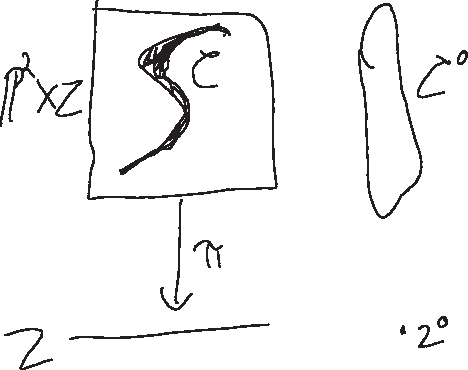
\includegraphics[width=0.5\textwidth]{2011-02-09_Diagram_001}\end{center}

        The \emph{fiber} $\mathcal C^0 = \pi^{-1}(z^0)$ of $\mathcal C$ over a point $z^0\in Z$ is the curve whose equation is the polynomial obtained.

        by substituting $z_\nu^0$ for $z_\nu$.  The 3 partial derivatives $F_x$, $F_y$, $F_z$ are polynomials in $x$, $y$, $z$, $\{z_\nu\}$ linear in $z_\nu$ and homogeneous of degree $d - 1$ in $x$, $y$, $z$.  They define some subvariety of $\mathbb P^2\times Z$.  Let $S$ be the variety $\{F_1 = F_2 = F_3 = 0\}$.  Note that $S \subset \mathcal C$ (by Euler).

        The fiber $\mathcal C^0$ over a point $z^0$ of $Z$ is smooth if and only if $\mathcal C^0$ doesn't meet $S$.

        We can construct $\Sigma = \pi(S)$ the image of $S$ via a polynomial $\mathbb P^2 \times Z \to Z$.  Later we'll prove that the image of the projection of any Zariski closed subvariety of $\mathbb P^2 \times Z$ to $Z$ is also Zariski closed.

        So the set $\Sigma$ is closed in the affine space $Z$.  But $\Sigma$ is not all of $Z$ (because the Fermat curve is smooth).  So $\Sigma \subset Z$ is a proper closed subvariety.  So the set of $z^0$ for which $\mathcal C^0$ is smooth is a Zariski open subset of $\mathbb A^N$.
      \end{proof}
\end {document}

